\documentclass[11pt]{article}

% ----------------------------------------------------------------------
%  geometry-gen : project report
%  Natural-language geometry problems -> renderable GeoGebra constructions
%  Compile:  pdflatex report.tex   (twice, for the ToC / references)
% ----------------------------------------------------------------------

\usepackage[a4paper,margin=1in]{geometry}
\usepackage[T1]{fontenc}
\usepackage{lmodern}
\usepackage{microtype}
\usepackage{amsmath,amssymb}
\usepackage{booktabs}
\usepackage{longtable}
\usepackage{enumitem}
\usepackage{xcolor}
\usepackage{listings}
\usepackage{graphicx}
\usepackage{caption}
\usepackage[hidelinks]{hyperref}
\usepackage{tikz}
\usetikzlibrary{arrows.meta,positioning,shapes.geometric}

% ---- code listing style -------------------------------------------------
\definecolor{codebg}{RGB}{247,248,250}
\definecolor{codekw}{RGB}{37,99,235}
\definecolor{codecm}{RGB}{107,114,128}
\definecolor{codestr}{RGB}{21,128,61}
\lstdefinestyle{mono}{
  backgroundcolor=\color{codebg},
  basicstyle=\ttfamily\footnotesize,
  keywordstyle=\color{codekw}\bfseries,
  commentstyle=\color{codecm}\itshape,
  stringstyle=\color{codestr},
  breaklines=true,
  showstringspaces=false,
  frame=single,
  framesep=5pt,
  rulecolor=\color{codebg},
  columns=fullflexible,
  keepspaces=true,
}
\lstset{style=mono}
\newcommand{\code}[1]{\texttt{\small #1}}

\title{\textbf{geometry-gen}\\[4pt]
\large Teaching a small language model to turn natural-language\\
Olympiad geometry problems into renderable GeoGebra constructions}
\author{Project report}
\date{\today}

\begin{document}
\maketitle

\begin{abstract}
\noindent
\textbf{geometry-gen} is an end-to-end experiment that fine-tunes a small,
laptop-runnable language model to translate a natural-language plane-geometry
problem into a machine-executable \emph{GeoGebra construction}: an ordered list
of construction steps that draws an interactive, draggable diagram of the
problem. The defining idea of the project is that a \emph{real geometry engine
is used as an automatic correctness oracle}. Every construction --- both the
training data and the model's output --- is rendered in a headless GeoGebra
engine and is accepted only if every step produces an object that exists; an
optional second layer probes the resulting coordinates and verifies that the
stated theorem holds numerically. This oracle is what makes the dataset
trustworthy and the evaluation faithful to production behaviour. We curate $82$
gold problems, programmatically grow the corpus to $232$ verified problems,
QLoRA-fine-tune \textbf{Qwen2.5-Coder-3B-Instruct} on the result, and evaluate
\emph{functionally} --- by rendering the model's predictions. On a held-out set
of $31$ problems the fine-tuned model produces schema-valid JSON $100\%$ of the
time and a construction that renders as a valid, non-degenerate figure $61\%$ of
the time before any repair, with a generate--validate--repair loop available to
recover further cases.
\end{abstract}

\tableofcontents
\bigskip\hrule

% =====================================================================
\section{Overview and motivation}
% =====================================================================

A geometry problem is usually accompanied by a figure. Producing a
\emph{correct, interactive} figure from the prose is itself hard: the diagram
must realise the stated constraints structurally (a midpoint must be a real
midpoint, an incircle must actually touch the sides), it must be
non-degenerate, and it must remain manipulable. geometry-gen treats this as a
\textbf{constrained code-generation} task: the target ``code'' is a JSON list of
native GeoGebra commands.

The central engineering principle is the use of GeoGebra itself as a
\textbf{verifier in the loop} at every stage:
\begin{enumerate}[nosep]
  \item to \emph{certify} the $82$ hand-curated seed problems;
  \item to \emph{gate} every machine-generated problem added to the corpus;
  \item to choose \emph{training labels} (which objects are shown vs. hidden);
  \item to \emph{filter} the model's output at inference time; and
  \item to \emph{score} the model with a functional metric that mirrors
        production.
\end{enumerate}
Because the model only needs to be good enough that a short
validate-and-repair loop reaches a renderable figure, a $3$B-parameter model
running in $4$-bit on a $6$\,GB GPU (or a laptop CPU) suffices.

\subsection{System at a glance}

\begin{center}
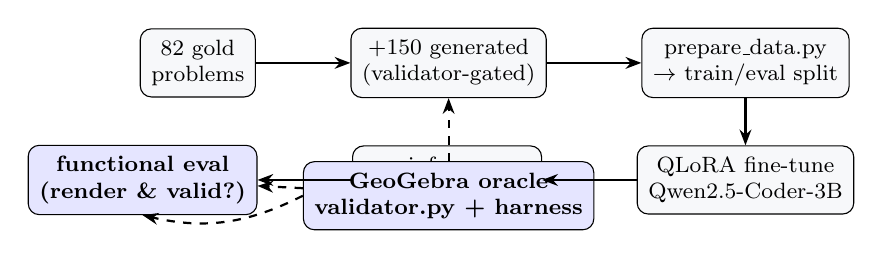
\begin{tikzpicture}[
  node distance=6mm and 12mm,
  box/.style={draw,rounded corners,align=center,font=\footnotesize,
              minimum height=8mm,inner sep=4pt,fill=codebg},
  ora/.style={draw,rounded corners,align=center,font=\footnotesize\bfseries,
              minimum height=8mm,inner sep=4pt,fill=blue!10},
  ar/.style={-{Stealth[length=2mm]},thick}]
\node[box] (gold) {$82$ gold\\problems};
\node[box,right=of gold] (gen) {$+150$ generated\\(validator-gated)};
\node[box,right=of gen] (prep) {prepare\_data.py\\$\to$ train/eval split};
\node[box,below=of prep] (train) {QLoRA fine-tune\\Qwen2.5-Coder-3B};
\node[box,left=of train] (infer) {infer.py\\predictions.jsonl};
\node[ora,left=of infer] (eval) {functional eval\\(render \& valid?)};
\node[ora,below=8mm of gen] (oracle) {GeoGebra oracle\\validator.py + harness};

\draw[ar] (gold) -- (gen);
\draw[ar] (gen) -- (prep);
\draw[ar] (prep) -- (train);
\draw[ar] (train) -- (infer);
\draw[ar] (infer) -- (eval);
\draw[ar,dashed] (oracle) -- (gen);
\draw[ar,dashed] (oracle) -- (eval);
\draw[ar,dashed] (oracle.west) to[bend left=20] (eval.south);
\end{tikzpicture}
\end{center}
\captionof{figure}{The same GeoGebra oracle (dashed) gates data generation and
scores the model.}

% =====================================================================
\section{Data representation}
% =====================================================================

\subsection{The construction schema}
Each problem is a single JSON object (one line of a JSONL file) with a
\code{problem\_statement} and an ordered \code{construction\_steps} array. Each
step has five fields:

\begin{center}
\begin{tabular}{@{}lp{11.4cm}@{}}
\toprule
\textbf{field} & \textbf{meaning}\\
\midrule
\code{name}    & unique identifier; later steps reference it. Steps execute
                 top-to-bottom, so a command may only use names defined earlier
                 (a constructible/topological order).\\
\code{type}    & \code{"final"} (shown) or \code{"construction"} (hidden helper /
                 scaffolding).\\
\code{class}   & \code{point\,|\,line\,|\,segment\,|\,ray\,|\,circle\,|\,conic\,|\,
                 number\,|\,angle\,|\,vector\,|\,list\,|\,locus\,|\,polygon}.\\
\code{label}   & optional display caption (e.g.\ $\Gamma$, $A'$).\\
\code{command} & native GeoGebra syntax: a coordinate literal \code{(0, 2)} for a
                 free point, or a command such as \code{Circle(O, 2)},
                 \code{Midpoint(B, C)}, \code{Intersect($\Gamma$, c, 2)},
                 \code{Reflect(H, O)}, \code{(A + B + C) / 3}.\\
\bottomrule
\end{tabular}
\end{center}

A worked example (the median construction, the centroid theorem):

\begin{lstlisting}[language=,]
{"id": 1,
 "problem_statement": "In triangle ABC let M, N, P be the midpoints of
   BC, CA, AB. Prove the medians AM, BN, CP are concurrent (centroid G) ...",
 "construction_steps": [
   {"name":"A","type":"final","class":"point","label":"A","command":"(-4, -2)"},
   {"name":"B","type":"final","class":"point","label":"B","command":"(5, -1)"},
   {"name":"C","type":"final","class":"point","label":"C","command":"(1, 5)"},
   {"name":"M","type":"final","class":"point","label":"M","command":"Midpoint(B, C)"},
   {"name":"N","type":"final","class":"point","label":"N","command":"Midpoint(C, A)"},
   {"name":"P","type":"final","class":"point","label":"P","command":"Midpoint(A, B)"},
   {"name":"median_A","type":"final","class":"segment","command":"Segment(A, M)"},
   ...
   {"name":"G","type":"final","class":"point","label":"G","command":"(A + B + C) / 3"}]}
\end{lstlisting}

\subsection{Free points on a path: the parameterisation trick}
A ``free point on circle $\omega$'' is written \code{Point(omega)}. If several
such points share one path, GeoGebra collapses them all onto the path's anchor.
The renderer/harness therefore auto-injects a parameter: the $i$-th of $k$
points sharing a path is placed at $t=(i+1)/(k+1)$, or (for robustness testing)
at a random value stratified into the slice $[\,i/k,(i+1)/k\,]$. Crucially the
point is created as a bare \code{Point(path)} and then \emph{nudged} to $t$ with
\code{SetValue}, so it stays \emph{draggable} --- writing \code{Point(path, t)}
directly would pin it. Points on infinite lines are excluded from this treatment
because the parameterised form there can become non-draggable.

\subsection{Datasets actually shipped}
\begin{center}
\begin{tabular}{@{}lrrl@{}}
\toprule
\textbf{file} & \textbf{problems} & \textbf{steps (min/med/max)} & \textbf{role}\\
\midrule
\code{geometry\_problems.jsonl}          & $82$  & $8\,/\,19\,/\,34$ & gold seed + style anchor\\
\code{datagen/generated\_problems.jsonl} & $150$ & $6\,/\,13\,/\,23$ & machine-grown corpus\\
\midrule
\textbf{total training pool}             & $232$ & --- & merged for fine-tuning\\
\bottomrule
\end{tabular}
\end{center}

\paragraph{Optional semantic checks.} Some problems carry a top-level
\code{checks} array asserting the theorem they illustrate, drawn from a rich
vocabulary: \code{collinear}, \code{concyclic}, \code{concurrent},
\code{parallel}, \code{perpendicular}, \code{equal\_len}, \code{on\_circle},
\code{midpoint}, \code{tangent\_circles}, \code{equal\_area},
\code{len\_product\_equal} (power of a point), \code{angle\_equal},
\code{angle\_double} (inscribed angle), \code{ptolemy}, and more. These are
verified numerically (Section~\ref{sec:oracle}).

% =====================================================================
\section{The GeoGebra oracle: renderer, harness, validator}
\label{sec:oracle}
% =====================================================================

\subsection{Renderer (\texttt{renderer.html})}
The human-facing tool: paste one problem's JSON, click \textbf{Render}, and a
full interactive GeoGebra ``classic'' applet (toolbar, input bar, zoom,
right-click properties) draws the figure with the statement shown above it. Key
behaviours: command success is judged by \code{exists(name)} \emph{after}
\code{evalCommand} (GeoGebra's return value is unreliable); points/circles get
labels but lines/segments/rays never do; \code{construction} objects are hidden
unless a checkbox reveals them; and \code{fitView()} forces a $1{:}1$ aspect
ratio so circles render as circles.

\subsection{Headless harness (\texttt{test\_harness.html})}
The UI-less twin that mirrors the renderer's logic exactly and is driven from
Python via Playwright/Chromium. It exposes \code{runSteps} (failures +
coordinates), \code{probeFull} (\emph{full-precision} coordinates for theorem
checking), \code{runProblemRandom} (random-$t$ build, failure count), and
\code{renderLikeApp} (drag-test that points stay manipulable). It signals
readiness via \code{window.\_\_ggbReady}.

\subsection{Validator and the robustness principle (\texttt{validator.py})}
\code{GeoGebraValidator} packages the oracle as a reusable context manager
(localhost server $+$ headless browser $+$ harness). A construction can render
cleanly for one lucky value of $t$; therefore the validator renders
\textbf{several times with fresh random $t$} and accepts only if \emph{every}
trial is clean:
\[
\text{accept} \iff \forall\, \text{trial}\in\{1,\dots,T\}:\;
\#\{\text{steps that failed to produce an object}\} = 0 .
\]
The same class is reused for data generation, inference filtering, the repair
loop, and evaluation --- so the gate is identical everywhere.

\subsection{Numeric theorem checks (\texttt{checks.py})}
Renderability is necessary but not sufficient: a \emph{wrong intersection-index}
pick can render fine yet be geometrically wrong. \code{checks.py} verifies the
stated theorem against the full-precision probed coordinates with a relative
tolerance $\tau = 10^{-6}\cdot(\text{figure scale})$. The key observation: a
\emph{true} theorem holds for all positions of the free points, whereas a wrong
construction is off by $O(1)$, so $\tau$ cleanly separates them.

% =====================================================================
\section{Data-generation pipeline (\texttt{datagen/})}
% =====================================================================

The aim is to grow the $82$ seed problems into hundreds \emph{without ever
admitting a problem that fails to render}.

\subsection{LLM generator (\texttt{generate.py})}
Claude (\code{claude-opus-4-8}, adaptive thinking) proposes one problem per call.
Design highlights:
\begin{itemize}[nosep]
  \item \textbf{Few-shot anchoring:} a fixed, diverse set of $10$ gold problems
        fixes schema and style.
  \item \textbf{Rules block:} encodes hard-won GeoGebra pitfalls (uppercase
        point names or a coordinate becomes a vector; \code{gamma} is reserved;
        incircle/circumcircle/center idioms; correct intersection index;
        tangents-from-a-point via a \code{\{Tangent(\dots)\}} list; no free point
        on an infinite line).
  \item \textbf{Prompt caching:} the $\sim$6k-token schema$+$rules$+$examples
        prefix sits in a cached system block; only a per-call theme and random
        nonce vary (after the cache point), so repeated calls re-read the prefix
        at $\sim$0.1$\times$ cost.
  \item \textbf{Validator-gated with one repair attempt:} each candidate is run
        through \code{validate\_robust}; on failure the failing steps are fed
        back once for a correction, which is re-validated. Only survivors are
        written; generated ids are marked $\ge 1000$.
\end{itemize}

\subsection{No-API path and filters}
\begin{description}[style=nextline,leftmargin=1.2em,nosep]
  \item[\texttt{validate\_candidates.py}] validates directly-authored candidates
    through two gates --- (1) renderability, (2) if \code{checks} are present,
    numeric theorem truth --- appending survivors, logging rejects with the
    failing step.
  \item[\texttt{post\_filter.py}] the \emph{inference-time} gate. A new problem
    has no ground-truth checks, so this applies generic degeneracy heuristics
    (points at infinity / non-finite; whole figure collapsed; too many coincident
    named points) and accepts by majority vote over trials (keep $\ge 60\%$
    clean). Includes lenient JSON repair for small-model syntax slips.
  \item[\texttt{visibility.py}] the ``show everything the statement names'' rule:
    promotes statement-referenced \code{construction} steps to \code{final}; used
    both to post-process inference output and to relabel training data so the
    model \emph{learns} the distinction.
  \item[\texttt{verify\_dataset.py}] read-only audit that re-renders every
    problem and re-checks every assertion from scratch.
  \item[\texttt{selftest.py}, \texttt{post\_filter\_selftest.py}] exercise the
    plumbing with no API key.
\end{description}

\subsection{Measured data quality}
Every shipped problem was re-audited with the oracle for this report:
\begin{center}
\begin{tabular}{@{}lrrl@{}}
\toprule
\textbf{dataset} & \textbf{problems} & \textbf{render-clean} & \textbf{trials}\\
\midrule
gold (\code{geometry\_problems.jsonl})      & $82$  & $82/82$ \ ($100\%$) & $8$ (all clean)\\
generated (\code{generated\_problems.jsonl})& $150$ & $150/150$ \ ($100\%$) & $5$ (all clean)\\
\bottomrule
\end{tabular}
\end{center}
\noindent Every problem in the corpus renders robustly across all random-$t$
trials --- the dataset is, by construction, $100\%$ valid.

% =====================================================================
\section{Fine-tuning pipeline (\texttt{finetune/})}
% =====================================================================

\subsection{Base model and hardware}
\begin{center}
\begin{tabular}{@{}ll@{}}
\toprule
Base model & \code{unsloth/Qwen2.5-Coder-3B-Instruct-bnb-4bit} (4-bit, $\sim$2\,GB)\\
Why        & code-specialised instruct model; largest that fits the target GPU\\
Hardware   & RTX 3050, $6$\,GB VRAM (fallback to 1.5B documented)\\
Template   & Qwen ChatML (\code{<|im\_start|>role \dots <|im\_end|>})\\
Toolchain  & Unsloth $+$ TRL \code{SFTTrainer} $+$ PEFT/bitsandbytes\\
\bottomrule
\end{tabular}
\end{center}

\subsection{Corpus preparation (\texttt{prepare\_data.py})}
The $232$ problems are relabelled with the visibility rule, converted to
three-message chat examples (system $\to$ schema instructions; user $\to$ problem
statement; assistant $\to$ the construction JSON), and split
\textbf{deterministically and stratified by source} (\code{seed=42},
$13\%$ eval) so the held-out set contains both gold and generated problems:
\[
\text{train} = 201,\qquad \text{eval} = 31\;(=11\ \text{gold} + 20\ \text{generated}).
\]
Three files result: \code{train.jsonl}, \code{eval.jsonl} (chat format), and
\code{eval\_problems.jsonl} (raw statements for functional eval).

\subsection{Training method: QLoRA}
The $3$B base is frozen and quantised to $4$-bit; small \textbf{LoRA} adapter
matrices are trained on top. Configuration:
\begin{center}
\begin{tabular}{@{}ll@{\hspace{2.2em}}ll@{}}
\toprule
LoRA rank $r$        & $16$            & max sequence length & $1536$\\
LoRA $\alpha$        & $16$            & epochs              & $4$\\
LoRA dropout         & $0$             & learning rate       & $2\times10^{-4}$, cosine\\
target modules       & all attn $+$ MLP proj. & warmup       & $5\%$\\
per-device batch     & $1$             & optimiser           & 8-bit AdamW\\
grad.\ accumulation  & $8$ (eff.\ batch $8$) & weight decay  & $0.01$\\
precision            & bf16/fp16 (auto)& seed                & $42$\\
\bottomrule
\end{tabular}
\end{center}
Target modules are \code{q\_proj, k\_proj, v\_proj, o\_proj, gate\_proj,
up\_proj, down\_proj}; Unsloth gradient checkpointing keeps activations within
$6$\,GB.

\subsection{Loss function and minimisation}
\label{sec:loss}
The objective is the standard \textbf{autoregressive cross-entropy}
(next-token) loss, computed \textbf{only over the assistant's JSON} --- the
prompt is masked out. For a target token sequence $y_1,\dots,y_N$ with the
model's predictive distribution $p_\theta$, the per-example loss is
\[
\mathcal{L}(\theta) \;=\; -\frac{1}{|\mathcal{R}|}
   \sum_{t\in\mathcal{R}} \log p_\theta\!\left(y_t \,\middle|\, y_{<t}\right),
\qquad
\mathcal{R} = \{\,t : y_t \text{ is part of the assistant response}\,\},
\]
where every token \emph{before} the assistant turn (the system prompt and the
user's problem statement) has its label set to the ignore index ($-100$) and
contributes nothing to $\mathcal{L}$. This is implemented with Unsloth's
\code{train\_on\_responses\_only} keyed on the ChatML markers
\code{<|im\_start|>user} and \code{<|im\_start|>assistant}. The model is thus
trained purely to \emph{emit the construction}, not to reproduce the prompt.

\medskip\noindent\textbf{How it is minimised.} Gradients
$\nabla_\theta \mathcal{L}$ flow \emph{only into the LoRA adapter weights}
(the quantised base is frozen). They are accumulated over $8$ micro-batches and
then applied by the \textbf{8-bit AdamW} optimiser; the learning rate follows a
\textbf{cosine decay} from $2\times10^{-4}$ after a $5\%$ linear warmup, across
$4$ epochs of the $201$ examples. Minimising $\mathcal{L}$ therefore means
adjusting the small low-rank matrices so the model places higher probability on
the correct construction-step tokens.

\medskip\noindent\textbf{Why no in-loop validation loss.} A full evaluation
forward materialises full-vocabulary fp32 logits ($\sim$2\,GB) and would
exhaust the $6$\,GB card, so \code{eval\_strategy="no"}. Model quality is judged
\emph{functionally} instead (Section~\ref{sec:results}): does the generated
construction actually render? Checkpoints are saved each epoch; final LoRA
adapters land in \code{qwen25coder3b-geom-lora/}.

\subsection{Inference, repair, and serving}
\begin{description}[style=nextline,leftmargin=1.2em,nosep]
  \item[\texttt{infer.py}] greedy decoding (\code{max\_new\_tokens}$=1280$) over
    the held-out set $\to$ \code{predictions.jsonl}.
  \item[\texttt{repair\_loop.py}] generate $\to$ validate $\to$ repair: failing
    constructions get the error fed back (up to $2$ retries), re-validated; loads
    the model at $8$k context because repair prompts are long. Reports accept
    rate before vs.\ after repair.
  \item[\texttt{eval\_predictions.py}] the functional metric
    (Section~\ref{sec:results}), run where GeoGebra is available.
  \item[\texttt{export\_gguf.py} / \texttt{geom.Modelfile} /
    \texttt{predict\_local.py}] merge LoRA $\to$ a single $4$-bit \code{q4\_k\_m}
    GGUF ($\sim$2\,GB) served by Ollama with JSON-grammar-constrained decoding,
    so the whole system runs on a laptop CPU with no GPU.
\end{description}

% =====================================================================
\section{Results}
\label{sec:results}
% =====================================================================

The metric that matters is \textbf{functional}: take the model's prediction for
each held-out problem and ask whether it (a) parses as schema-valid JSON and
(b) renders as a valid, non-degenerate figure under the production
\code{post\_filter} gate ($7$ random-$t$ trials). Measured on the $31$ held-out
problems:

\begin{center}
\begin{tabular}{@{}lrr@{}}
\toprule
\textbf{metric} & \textbf{count} & \textbf{rate}\\
\midrule
parseable schema JSON               & $31/31$ & $100\%$\\
renders \& valid (before repair)    & $19/31$ & $61\%$\\
renders \& valid \,$|$\, parseable  & $19/31$ & $61\%$\\
\bottomrule
\end{tabular}
\end{center}

\paragraph{Reading the numbers.} The model has fully internalised the
\emph{schema}: every prediction is well-formed JSON in the right shape ($100\%$).
The harder skill --- emitting a construction that is \emph{geometrically
executable} --- succeeds outright $61\%$ of the time. The remaining $39\%$ fail
for diagnosable, recurring reasons rather than malformed output, which is
exactly what the repair loop targets.

\subsection{Failure taxonomy}
The $12$ failures on the held-out set group into three causes:
\begin{center}
\begin{tabular}{@{}lp{8.6cm}r@{}}
\toprule
\textbf{cause} & \textbf{example error} & \textbf{share}\\
\midrule
undefined / mis-cased name or bad command &
  \code{Line\_B\_C} used but never defined; \code{tangent(\dots)} lowercase;
  \code{Midpoint(line)} on a line &  majority\\
point at infinity (\code{nan}) &
  parallel-line intersection $\Rightarrow$ \code{(nan, nan)} &  several\\
degenerate collapse &
  too many coincident points (e.g.\ ``$3$ distinct of $9$'') &  a few\\
\bottomrule
\end{tabular}
\end{center}
These are precisely the error classes the repair instruction addresses (``define
every name before use; exact GeoGebra casing; avoid points at infinity''), so
the $61\%$ figure is a \emph{lower bound} on what the full
generate--validate--repair system delivers; \code{repair\_loop.py} exists to
recover the recoverable cases by re-prompting with the exact error.

\subsection{What the result demonstrates}
\begin{itemize}[nosep]
  \item A $3$B model, QLoRA-tuned on only $201$ verified examples, learns the
        target DSL well enough to produce a directly-renderable Olympiad figure
        for the majority of unseen problems.
  \item Schema adherence is effectively solved ($100\%$), so the residual error
        is purely \emph{geometric/semantic} --- the tractable part, addressable
        by the in-the-loop verifier.
  \item The oracle-in-the-loop design means a modest raw accuracy is amplified
        by automatic validation and repair into a usable end-to-end tool.
\end{itemize}

% =====================================================================
\section{Limitations and honest caveats}
% =====================================================================
\begin{itemize}[nosep]
  \item \textbf{Renderability $\ne$ truth at inference.} The production
        \code{post\_filter} checks that a figure draws and is non-degenerate, not
        that it proves the stated theorem. The numeric \code{checks} oracle
        closes this gap but needs a ground-truth assertion, which unseen problems
        lack. (One shipped prediction renders yet pairs the wrong intersection
        points --- valid figure, wrong geometry.)
  \item \textbf{Repository snapshots vs.\ code.} The shipped
        \code{generated\_problems.jsonl} is renumbered $1$--$150$ with no
        \code{checks}, whereas the generation code assumes ids $\ge1000$ with
        semantic checks; one training docstring still says ``7B'' though the
        config trains $3$B. These are documentation/snapshot mismatches, not
        logic errors.
  \item \textbf{Small held-out set.} $31$ problems give a clear signal but a wide
        confidence interval; the $61\%$ figure should be read as indicative.
  \item \textbf{Model weights excluded.} The $\sim$2\,GB GGUF is gitignored, so
        the repository is reproducible from scripts but does not embed the
        trained model.
\end{itemize}

% =====================================================================
\section{Reproduction summary}
% =====================================================================
\begin{enumerate}[nosep]
  \item \textbf{Validate the seed:} \code{python validate.py} ($82/82$ clean).
  \item \textbf{Grow the corpus:} \code{python datagen/generate.py --n N}
        (API) or \code{validate\_candidates.py} (no API); audit with
        \code{verify\_dataset.py}.
  \item \textbf{Prepare data:} \code{python finetune/prepare\_data.py}
        $\to$ train/eval split.
  \item \textbf{Train (GPU box):} \code{python finetune/qlora\_train.py}
        $\to$ LoRA adapters.
  \item \textbf{Predict \& repair:} \code{infer.py}, \code{repair\_loop.py}.
  \item \textbf{Score (where GeoGebra runs):}
        \code{python finetune/eval\_predictions.py --trials 7}.
  \item \textbf{Serve locally:} \code{export\_gguf.py} $\to$ Ollama
        (\code{geom.Modelfile}) $\to$ \code{predict\_local.py} $\to$ paste JSON
        into \code{renderer.html}.
\end{enumerate}

\bigskip\hrule\medskip
\noindent\footnotesize All quantitative results in this report were produced by
re-running the project's own validation harness ($\code{validate.py}$,
$\code{datagen/verify\_dataset.py}$, $\code{finetune/eval\_predictions.py}$) on
the committed data and predictions.

\end{document}
